\chapter{KẾT QUẢ THỰC HIỆN VÀ PHÂN TÍCH DỮ LIỆU}

\section{Sản phẩm đã xây dựng}

Nhóm đã hoàn thành hệ thống dashboard trực quan hóa dữ liệu World Happiness Report. Sản phẩm gồm một trang chủ và năm trang phân tích chính. Dữ liệu được nạp trực tiếp từ năm tệp CSV năm 2015, 2016, 2017, 2018 và 2019 trong thư mục \textit{data}.

Trang chủ giới thiệu mục tiêu của dự án, hiển thị năm dữ liệu mới nhất, số quốc gia, điểm hạnh phúc trung bình và số khu vực. Từ trang chủ, người dùng có thể điều hướng đến các trang Overview, Trends, Regional Analysis, Key Factors và Advanced Insights.

\section{Kết quả tiền xử lý dữ liệu}

\subsection{Chuẩn hóa cấu trúc dữ liệu}

Qua quá trình tiền xử lý, dữ liệu từ các năm được hợp nhất theo cấu trúc chung gồm quốc gia, khu vực, thứ hạng hạnh phúc, điểm hạnh phúc, GDP bình quân đầu người, hỗ trợ xã hội, tuổi thọ khỏe mạnh, tự do, sự hào phóng, nhận thức về tham nhũng và năm báo cáo.

Các cột có tên khác nhau giữa các năm đã được đổi thành tên thống nhất. Chẳng hạn, \textit{Country or region}, \textit{Overall rank}, \textit{Score}, \textit{Economy (GDP per Capita)} và \textit{Health (Life Expectancy)} được ánh xạ tương ứng về \textit{Country}, \textit{Happiness Rank}, \textit{Happiness Score}, \textit{GDP per capita} và \textit{Life Expectancy}.

\subsection{Quy mô dữ liệu}

\begin{table}[H]
\centering
\begin{tabular}{|c|c|c|}
\hline
\textbf{Năm} & \textbf{Số quốc gia} & \textbf{Điểm hạnh phúc trung bình} \\
\hline
2015 & 158 & 5.3757 \\
\hline
2016 & 157 & 5.3822 \\
\hline
2017 & 155 & 5.3540 \\
\hline
2018 & 156 & 5.3759 \\
\hline
2019 & 156 & 5.4071 \\
\hline
\end{tabular}
\caption{Quy mô dữ liệu theo từng năm}
\label{tab:quy-mo-du-lieu}
\end{table}

Bảng \ref{tab:quy-mo-du-lieu} cho thấy quy mô dữ liệu ổn định trong giai đoạn nghiên cứu, dao động từ 155 đến 158 quốc gia mỗi năm. Điểm hạnh phúc trung bình của toàn bộ quan sát năm 2015--2019 dao động trong khoảng 5.3540--5.4071, vì vậy biên độ thay đổi trung bình qua các năm không lớn.

\section{Kết quả trang tổng quan theo năm}

Trang Overview cho phép người dùng chọn từng năm và xem dữ liệu của năm đó. Đối với năm 2019, hệ thống hiển thị 156 quốc gia và chia dữ liệu thành các khu vực địa lý. Người dùng có thể chọn khu vực trên quả địa cầu trực giao để làm nổi bật khu vực tương ứng; bảng dữ liệu bên dưới sẽ được lọc theo khu vực đã chọn.

Các quốc gia có điểm hạnh phúc cao nhất năm 2019 gồm Phần Lan, Đan Mạch, Na Uy, Iceland và Hà Lan. Trong khi đó, Nam Sudan, Cộng hòa Trung Phi, Afghanistan, Tanzania và Rwanda nằm trong nhóm có điểm thấp nhất.

\begin{table}[H]
\centering
\begin{tabular}{|p{5.2cm}|c|p{5.2cm}|c|}
\hline
\multicolumn{2}{|c|}{\textbf{Nhóm điểm cao}} & \multicolumn{2}{c|}{\textbf{Nhóm điểm thấp}} \\
\hline
\textbf{Quốc gia} & \textbf{Điểm} & \textbf{Quốc gia} & \textbf{Điểm} \\
\hline
Finland & 7.769 & South Sudan & 2.853 \\
\hline
Denmark & 7.600 & Central African Republic & 3.083 \\
\hline
Norway & 7.554 & Afghanistan & 3.203 \\
\hline
Iceland & 7.494 & Tanzania & 3.231 \\
\hline
Netherlands & 7.488 & Rwanda & 3.334 \\
\hline
\end{tabular}
\caption{Nhóm quốc gia tiêu biểu năm 2019}
\label{tab:quoc-gia-tieu-bieu}
\end{table}

Biểu hiện của bản đồ và bảng dữ liệu hỗ trợ người dùng chuyển đổi nhanh giữa góc nhìn toàn cầu và góc nhìn khu vực. Lựa chọn khu vực không làm thay đổi dữ liệu gốc mà chỉ lọc các bản ghi phù hợp trong giao diện.

\section{Kết quả phân tích xu hướng}

\subsection{Xu hướng điểm hạnh phúc trung bình}

Trang Trends tính trung bình điểm hạnh phúc, GDP bình quân đầu người và tuổi thọ khỏe mạnh theo từng năm. Kết quả cho thấy điểm hạnh phúc trung bình từ năm 2015 đến 2019 có xu hướng dao động nhẹ:

\begin{itemize}
    \item Năm 2015: 5.3757.
    \item Năm 2016: 5.3822.
    \item Năm 2017: 5.3540.
    \item Năm 2018: 5.3759.
    \item Năm 2019: 5.4071.
\end{itemize}

So với năm 2015, điểm trung bình năm 2019 tăng khoảng 0.0314 điểm. Tuy nhiên, mức tăng này nhỏ và không biểu thị sự cải thiện lớn hay đồng đều ở tất cả quốc gia. Năm 2017 là năm có điểm trung bình thấp nhất trong giai đoạn được khảo sát.

Biểu đồ cho thấy năm 2017 có điểm trung bình thấp nhất, sau đó tăng dần đến mức cao nhất vào năm 2019. Các nhãn số trên từng điểm giúp đối chiếu chính xác giá trị. Trục tung trong hình được thu hẹp để làm rõ biến động nhỏ, không bắt đầu từ 0; vì vậy hình dạng đường không đại diện cho mức thay đổi trên toàn bộ thang điểm.

\begin{figure}[H]
\centering
\caption{Xu hướng điểm hạnh phúc trung bình giai đoạn 2015--2019}
\label{fig:xu-huong-hanh-phuc}
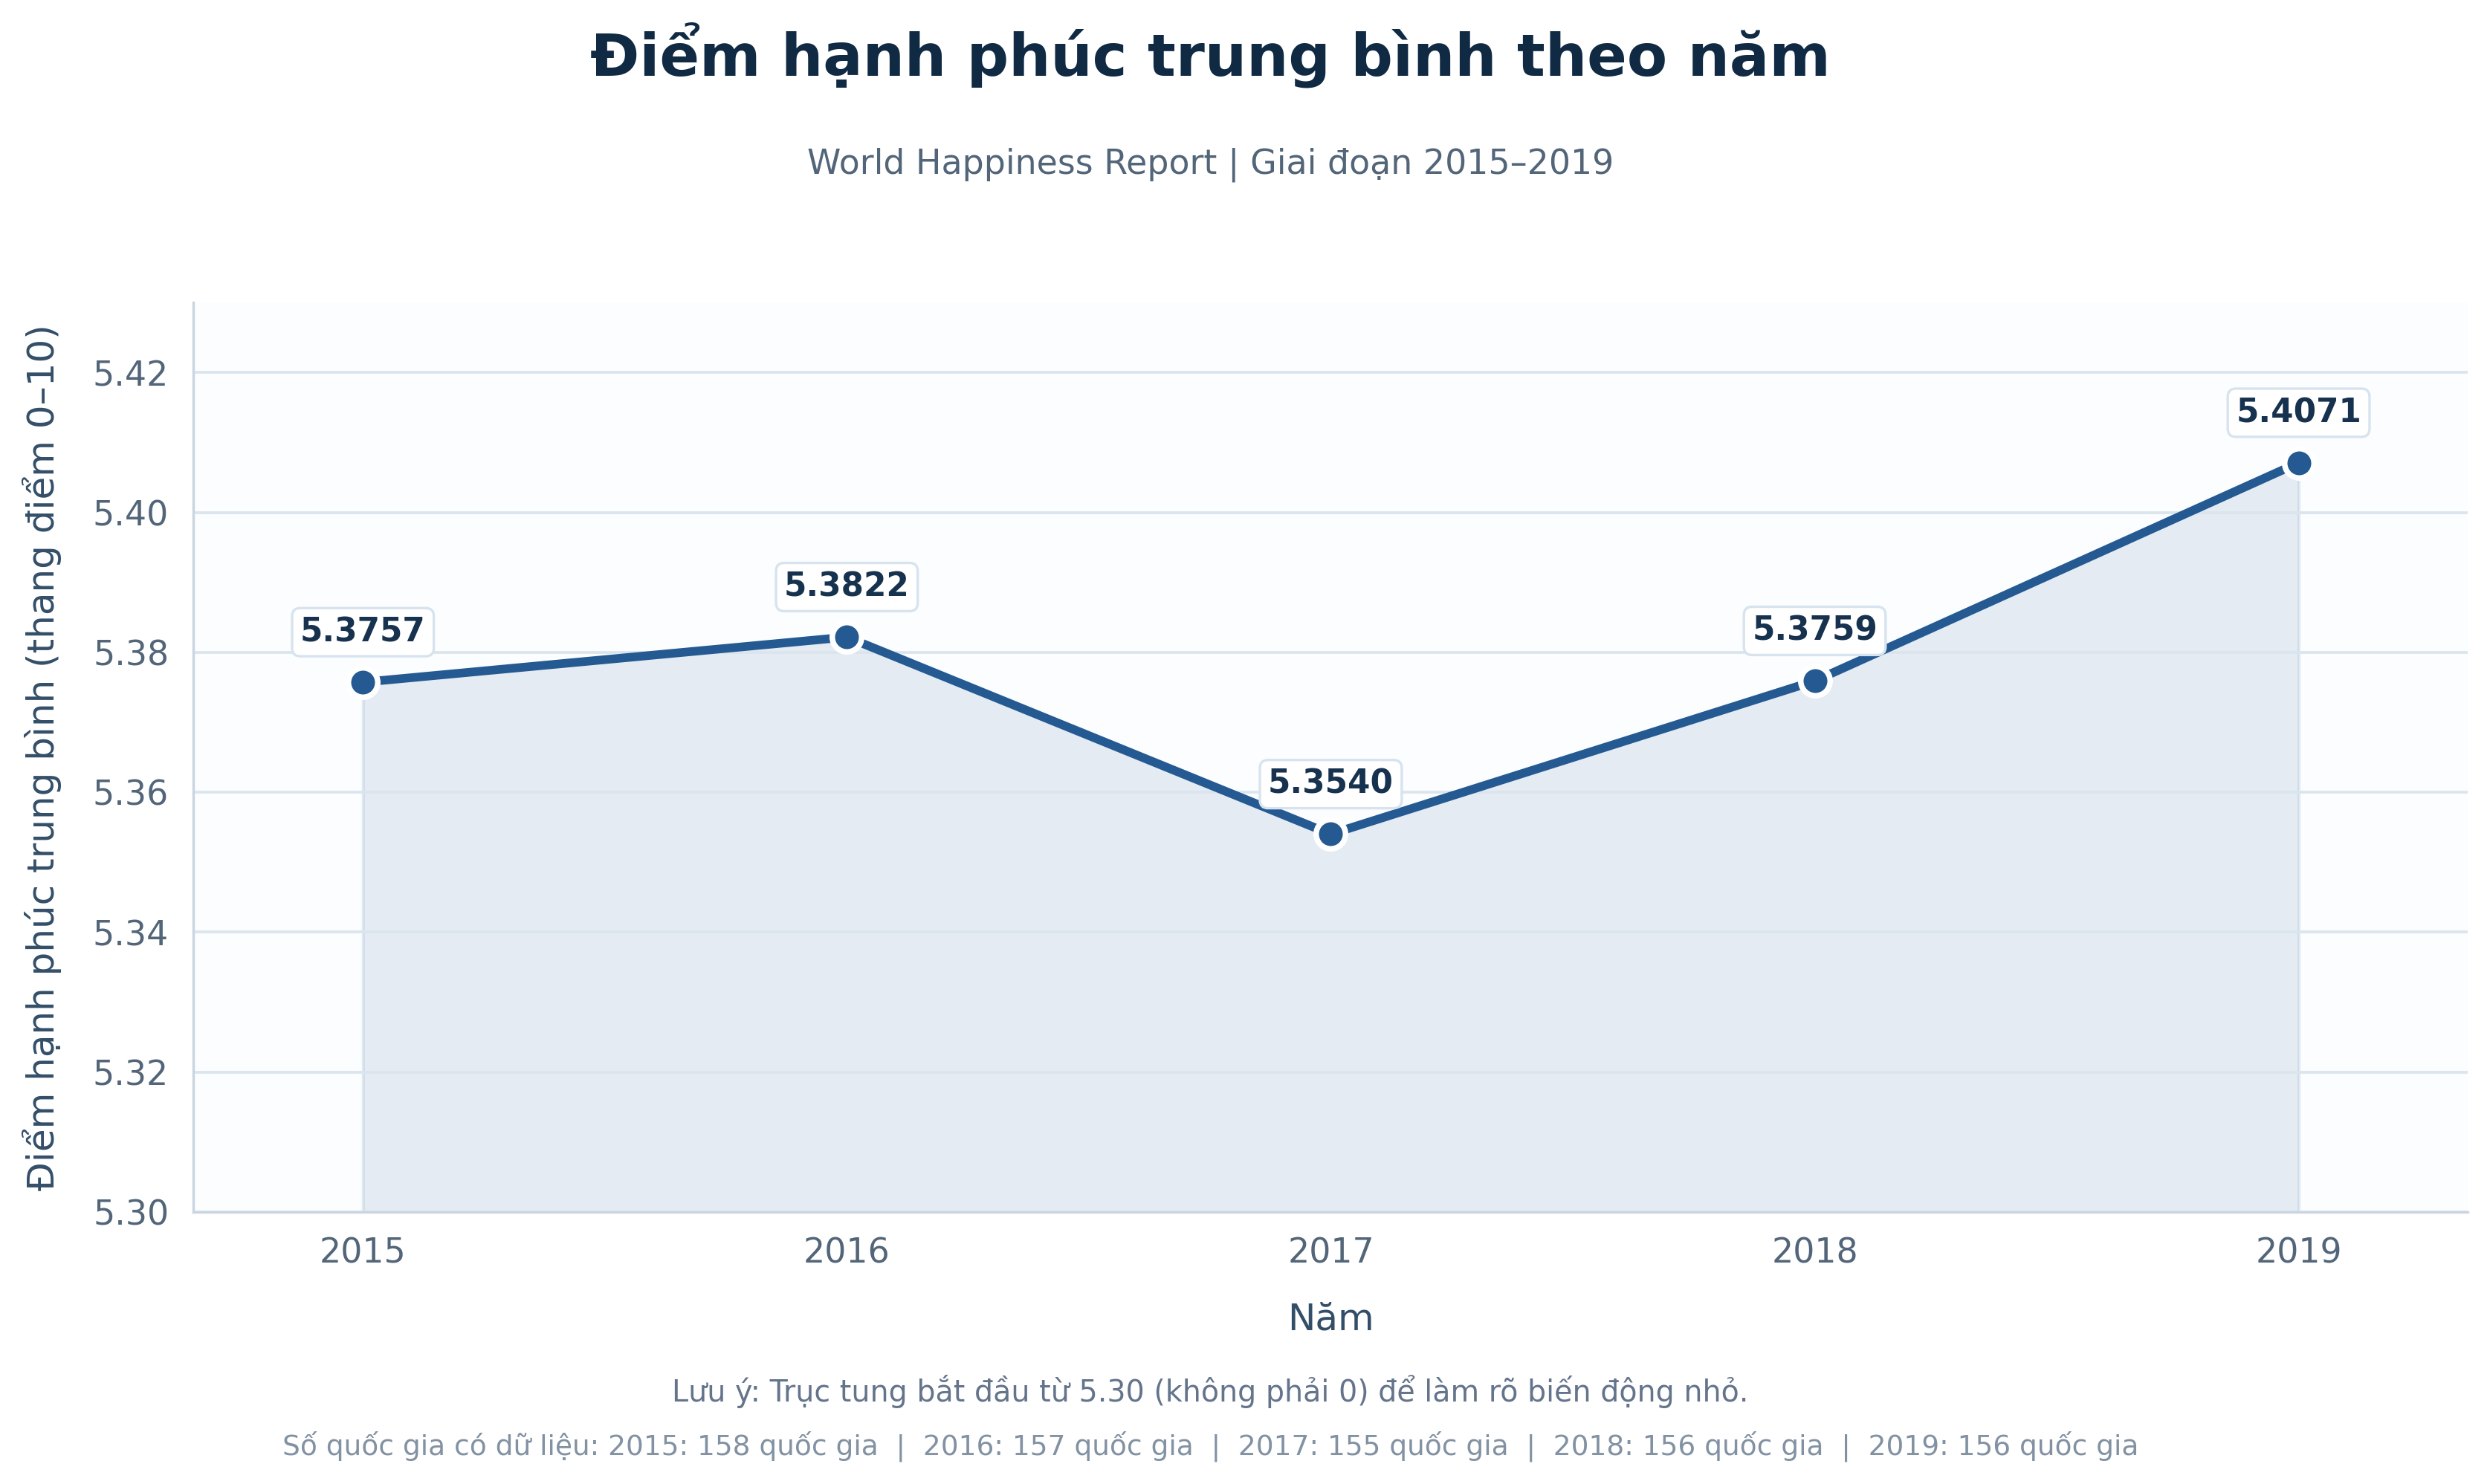
\includegraphics[width=0.88\textwidth]{images/bieu-do-xu-huong-hanh-phuc.png}
\end{figure}

\subsection{Tương quan giữa GDP, tuổi thọ và điểm hạnh phúc}

Biểu đồ phân tán cho phép người dùng chọn GDP bình quân đầu người hoặc tuổi thọ khỏe mạnh làm trục ngang. Khi lọc từng năm, hệ thống tính hệ số tương quan Pearson giữa trục đã chọn và điểm hạnh phúc.

Với toàn bộ giai đoạn 2015--2019, hệ số tương quan giữa GDP bình quân đầu người và điểm hạnh phúc là khoảng 0.789. Tương quan này thuộc mức mạnh theo chiều dương, nghĩa là các quốc gia có GDP bình quân đầu người cao nhìn chung cũng có xu hướng có điểm hạnh phúc cao hơn.

Tuổi thọ khỏe mạnh cũng có tương quan dương mạnh với điểm hạnh phúc. Kết quả này cho thấy điều kiện kinh tế và sức khỏe có liên hệ đáng kể với mức hạnh phúc trong dữ liệu nhưng không thể chứng minh rằng GDP hoặc tuổi thọ là nguyên nhân duy nhất của hạnh phúc.

\section{Kết quả phân tích theo khu vực}

Trang Regional Analysis tính điểm hạnh phúc trung bình và số quốc gia cho mỗi khu vực trong năm được chọn. Với dữ liệu năm 2019, Australia and New Zealand và North America là hai khu vực có điểm trung bình cao nhất trong các nhóm đủ dữ liệu.

\begin{table}[H]
\centering
\begin{tabular}{|p{6.2cm}|c|c|}
\hline
\textbf{Khu vực} & \textbf{Điểm trung bình} & \textbf{Số quốc gia} \\
\hline
Australia and New Zealand & 7.2675 & 2 \\
\hline
North America & 7.0850 & 2 \\
\hline
Western Europe & 6.8422 & 21 \\
\hline
Latin America and Caribbean & 5.9544 & 21 \\
\hline
Eastern Asia & 5.6888 & 6 \\
\hline
Central and Eastern Europe & 5.5615 & 29 \\
\hline
Southeastern Asia & 5.2737 & 9 \\
\hline
Middle East and Northern Africa & 5.2370 & 19 \\
\hline
Southern Asia & 4.5269 & 7 \\
\hline
Sub-Saharan Africa & 4.3001 & 40 \\
\hline
\end{tabular}
\caption{Điểm hạnh phúc trung bình theo khu vực năm 2019}
\label{tab:khu-vuc-2019}
\end{table}

Cần lưu ý rằng số quốc gia trong mỗi khu vực khác nhau. Vì vậy, điểm trung bình của khu vực có hai quốc gia chỉ phản ánh chính xác nhóm nhỏ này trong dữ liệu, không nên suy rộng thành kết luận về toàn bộ dân số khu vực.

\begin{figure}[H]
\centering
\caption{So sánh điểm hạnh phúc trung bình theo khu vực năm 2019}
\label{fig:khu-vuc-2019}
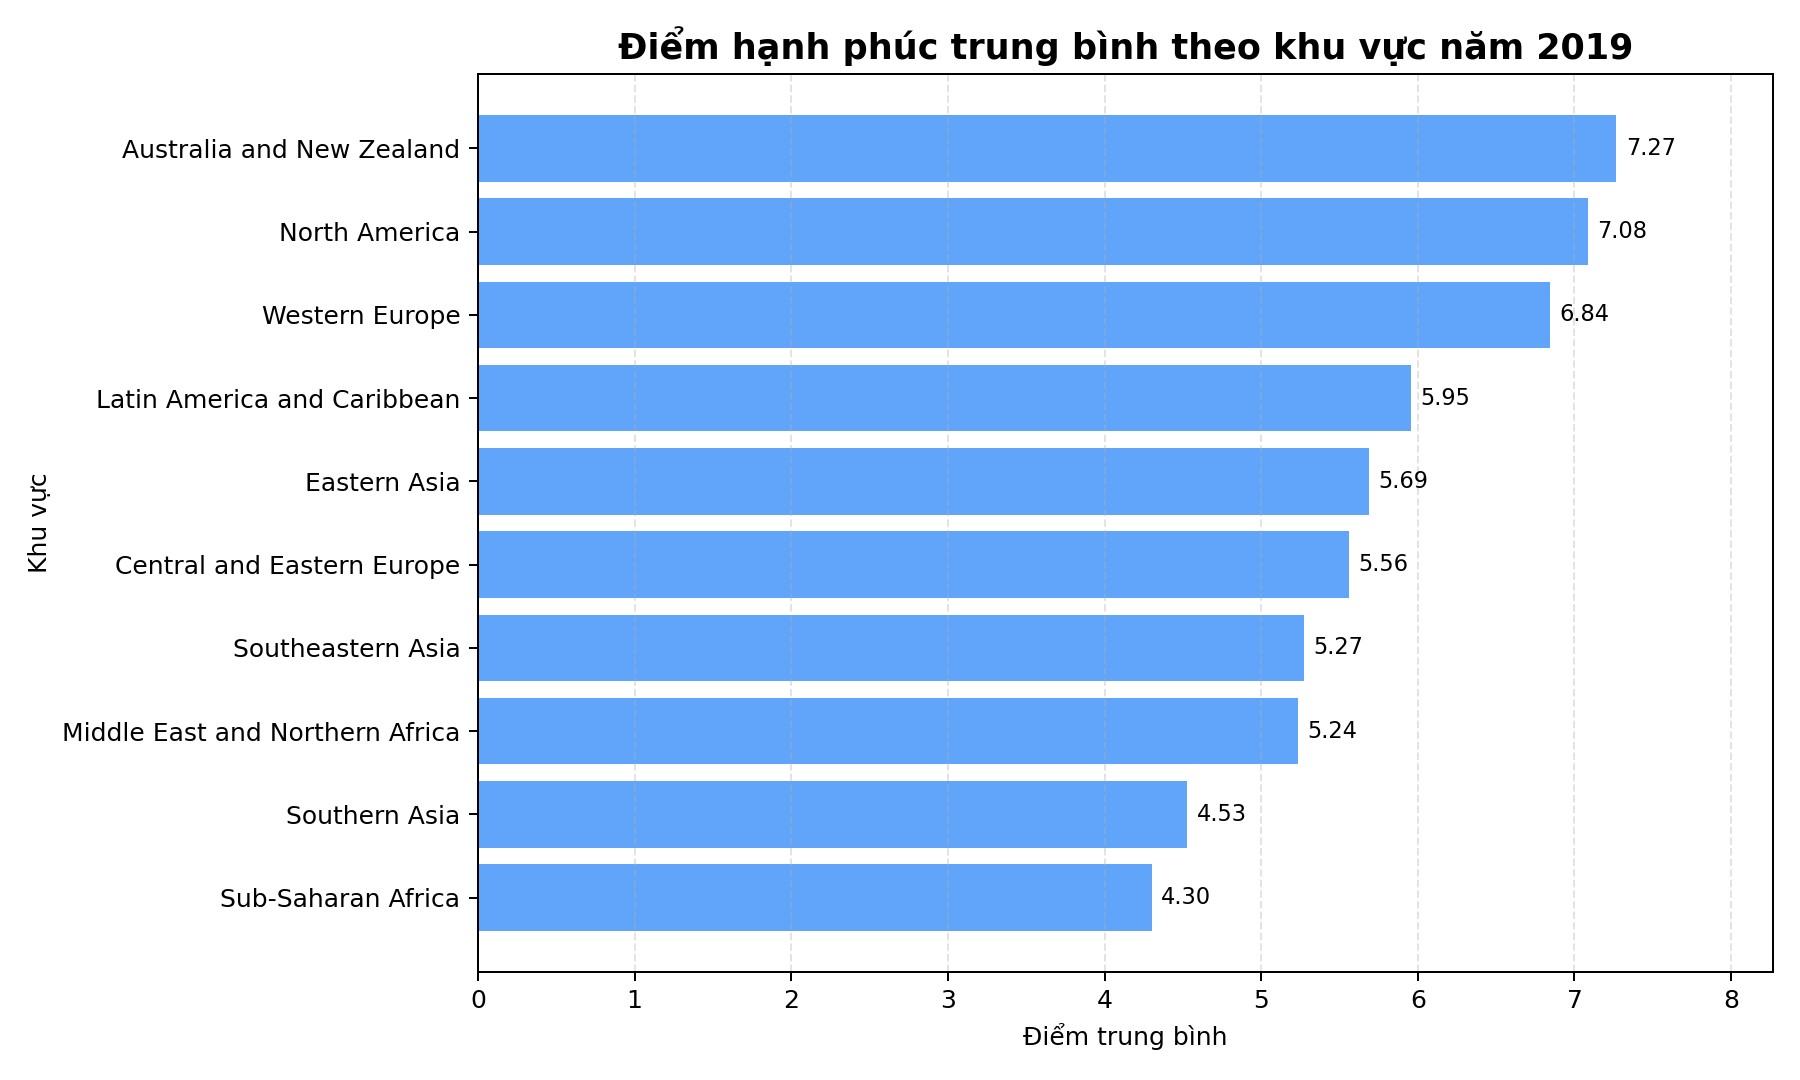
\includegraphics[width=0.90\textwidth]{images/bieu-do-khu-vuc-2019.png}
\end{figure}

Trang khu vực còn hỗ trợ chọn nhiều quốc gia để so sánh điểm hạnh phúc theo từng năm. Khi chọn ít nhất hai quốc gia, ứng dụng tạo biểu đồ đường với trục ngang là năm và trục dọc là điểm hạnh phúc. Chức năng này giúp nhận biết quốc gia tăng, giảm hay duy trì điểm số tương đối ổn định.

\section{Kết quả phân tích các yếu tố hạnh phúc}

\subsection{Ma trận tương quan}

Trang Key Factors tính ma trận tương quan Pearson giữa điểm hạnh phúc và các yếu tố GDP bình quân đầu người, hỗ trợ xã hội, tuổi thọ khỏe mạnh, tự do, hào phóng và nhận thức về tham nhũng.

Với toàn bộ dữ liệu giai đoạn 2015--2019, các hệ số tương quan với điểm hạnh phúc được sắp xếp như sau:

\begin{itemize}
    \item GDP bình quân đầu người: 0.7893.
    \item Tuổi thọ khỏe mạnh: 0.7425.
    \item Hỗ trợ xã hội: 0.6488.
    \item Tự do lựa chọn cuộc sống: 0.5513.
    \item Nhận thức về tham nhũng: 0.3973.
    \item Sự hào phóng: 0.1376.
\end{itemize}

\begin{table}[H]
\centering
\begin{tabular}{|p{6cm}|c|p{4cm}|}
\hline
\textbf{Yếu tố} & \textbf{Hệ số $r$} & \textbf{Mức liên hệ tuyến tính} \\
\hline
GDP per capita & 0.7893 & Mạnh, cùng chiều \\
\hline
Life Expectancy & 0.7425 & Mạnh, cùng chiều \\
\hline
Social support & 0.6488 & Vừa đến mạnh \\
\hline
Freedom & 0.5513 & Vừa \\
\hline
Perceptions of corruption & 0.3973 & Yếu đến vừa \\
\hline
Generosity & 0.1376 & Rất yếu \\
\hline
\end{tabular}
\caption{Tương quan Pearson với điểm hạnh phúc}
\label{tab:tuong-quan-yếu-to}
\end{table}

Kết quả cho thấy GDP bình quân đầu người có liên hệ tuyến tính mạnh nhất trong các yếu tố được khảo sát, tiếp theo là tuổi thọ khỏe mạnh và hỗ trợ xã hội. Sự hào phóng có hệ số dương nhưng liên hệ tuyến tính rất yếu.

\begin{figure}[H]
\centering
\caption{Tương quan Pearson giữa các yếu tố và điểm hạnh phúc}
\label{fig:tuong-quan-yeu-to}
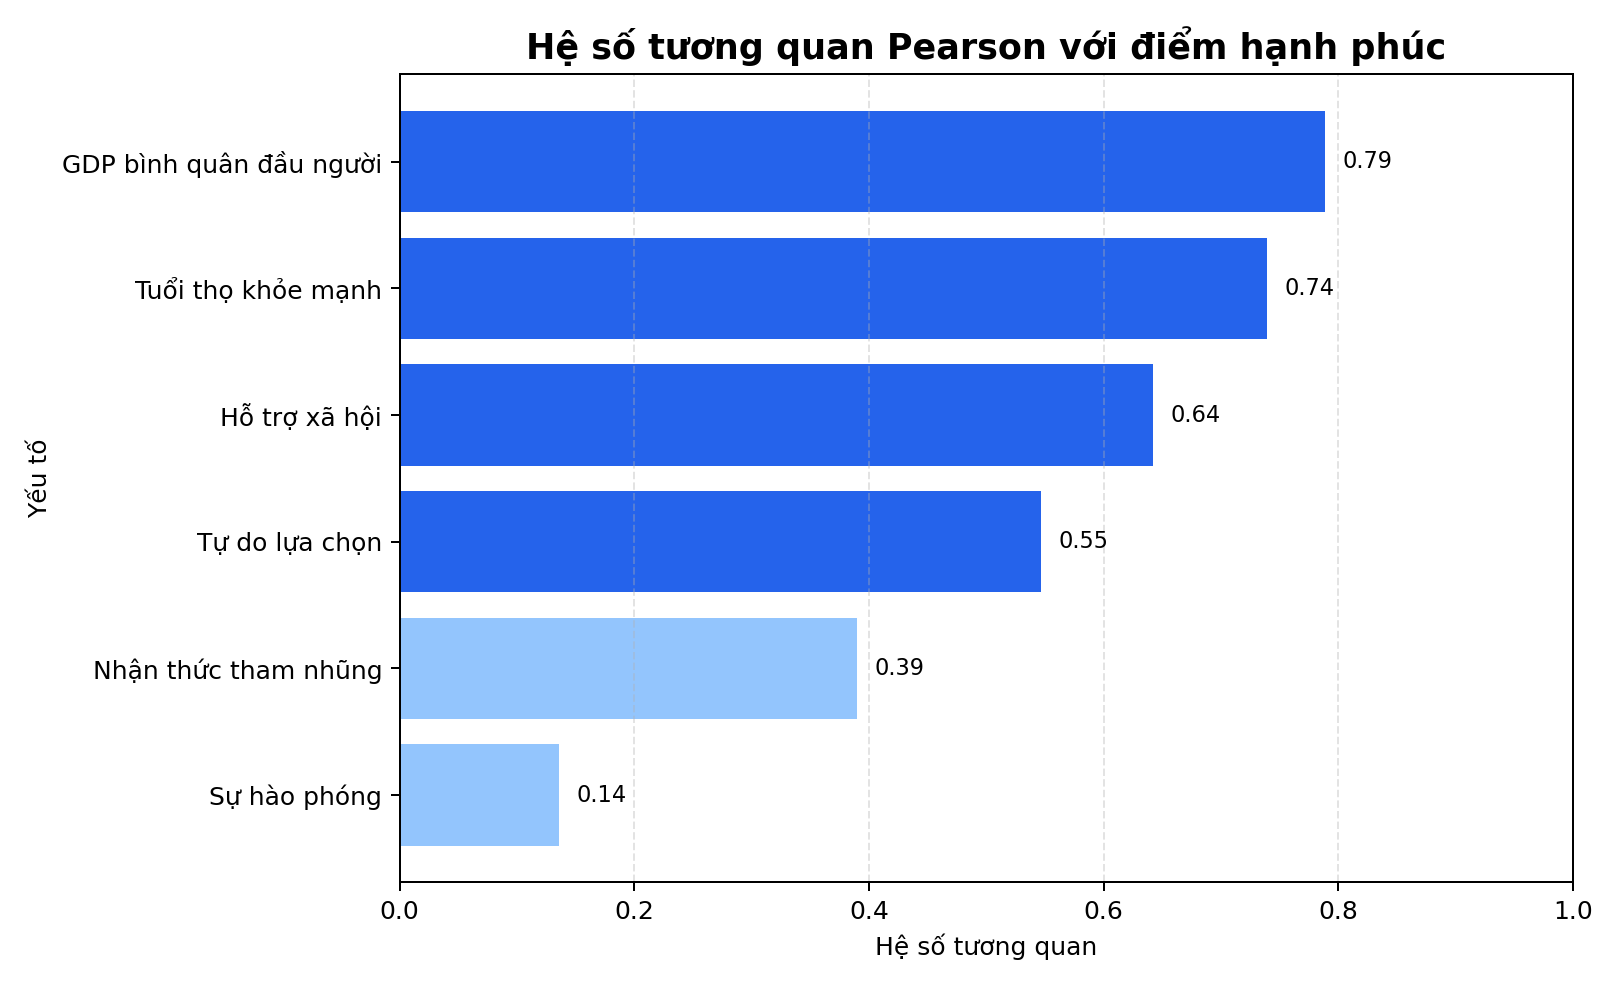
\includegraphics[width=0.88\textwidth]{images/bieu-do-tuong-quan-yeu-to.png}
\end{figure}

Ma trận tương quan cũng cho thấy các yếu tố kinh tế và xã hội thường có xu hướng liên quan với nhau. Tuy nhiên, hệ số tương quan không thể được dùng để khẳng định một yếu tố là nguyên nhân trực tiếp làm thay đổi điểm hạnh phúc.

\subsection{Pairplot các yếu tố}

Pairplot được xây dựng cho các chỉ số được người dùng chọn. Biểu đồ sử dụng điểm hạnh phúc, GDP, hỗ trợ xã hội, tuổi thọ hoặc các yếu tố khác để tạo ma trận phân tán. Màu sắc thể hiện khu vực địa lý.

Khi quan sát GDP và điểm hạnh phúc, các điểm có xu hướng phân bố theo đường tăng chung. Các quan sát tương tự xuất hiện ở cặp hỗ trợ xã hội -- điểm hạnh phúc và tuổi thọ -- điểm hạnh phúc. Ngược lại, cặp hào phóng -- điểm hạnh phúc có phân bố phân tán hơn và ít thể hiện xu hướng tuyến tính.

\section{Kết quả khám phá nâng cao}

Trang Advanced Insights cung cấp bộ lọc theo năm, khoảng điểm hạnh phúc và quốc gia. Dữ liệu sau khi lọc được cập nhật đồng thời cho ba tab Khám phá, So sánh và Yếu tố.

Trong tab Khám phá, người dùng có thể chọn yếu tố đặt ở trục ngang và quan sát phân tán với điểm hạnh phúc. Tab này còn hiển thị top 10 quốc gia có điểm cao nhất trong năm mới nhất thuộc phạm vi bộ lọc.

Trong tab So sánh, người dùng có thể chọn tối đa 8 quốc gia. Hệ thống vẽ đường biến động điểm hạnh phúc theo năm cho từng quốc gia, đồng thời hiển thị nhận xét về điểm cao nhất, điểm thấp nhất và mức thay đổi từ năm đầu đến năm cuối.

Trong tab Yếu tố, ứng dụng tính tương quan của từng yếu tố với điểm hạnh phúc trong phạm vi đang lọc. Người dùng có thể xác định yếu tố có tương quan mạnh nhất hoặc yếu tố cần quan sát thêm mà không thay đổi dữ liệu gốc.

\section{Đánh giá chức năng và chất lượng hệ thống}

\subsection{Ưu điểm}

\begin{itemize}
    \item Giao diện được chia thành nhiều trang theo mục tiêu phân tích rõ ràng.
    \item Dữ liệu được chuẩn hóa và có thể xem theo năm, khu vực, quốc gia hoặc khoảng điểm.
    \item Các biểu đồ hỗ trợ tương tác, đặt trỏ chuột để xem thông tin chi tiết và thay đổi phạm vi quan sát.
    \item Hệ thống kết hợp thống kê mô tả, tương quan và trực quan hóa trong một dashboard.
    \item Nhóm thống nhất cách đặt tên dữ liệu để tránh khác biệt giữa các tệp năm.
\end{itemize}

\subsection{Hạn chế}

\begin{itemize}
    \item Dữ liệu chỉ bao gồm giai đoạn 2015--2019 nên chưa phản ánh các năm gần đây hơn.
    \item Một số tên quốc gia và khu vực có thể thay đổi hoặc không thống nhất hoàn toàn giữa các năm.
    \item Tương quan Pearson chủ yếu đo quan hệ tuyến tính nên không phản ánh mọi dạng quan hệ phi tuyến.
    \item Dashboard chưa thực hiện mô hình dự đoán hoặc phân tích nhân quả.
    \item Một số trang mới có dữ liệu và nhận xét tự động, nhưng vẫn có thể cần bổ sung bài kiểm tra tự động cho toàn bộ quy trình.
\end{itemize}

\section{Kết quả đạt được}

Nhóm đã hoàn thành hệ thống trực quan đáp ứng các yêu cầu cơ bản:

\begin{enumerate}
    \item Tải và chuẩn hóa năm tệp dữ liệu World Happiness Report.
    \item Xây dựng trang chủ và các trang phân tích thống nhất giao diện.
    \item Hiển thị dữ liệu theo năm và theo khu vực trên bản đồ.
    \item Xây dựng biểu đồ xu hướng, vùng, phân tán, cột và heatmap.
    \item Tính hệ số tương quan Pearson và thống kê mô tả.
    \item Hỗ trợ lọc dữ liệu theo năm, khu vực, quốc gia và khoảng điểm hạnh phúc.
    \item So sánh nhiều quốc gia qua các năm báo cáo.
    \item Rút ra nhận xét dựa trên dữ liệu trong từng trang dashboard.
\end{enumerate}

\section{Hướng phát triển}

Trong thời gian tiếp theo, hệ thống có thể được mở rộng theo các hướng sau:

\begin{itemize}
    \item Cập nhật dữ liệu của các năm gần đây hơn.
    \item Bổ sung hồi quy tuyến tính hoặc mô hình học máy để dự đoán điểm hạnh phúc.
    \item Thêm phân cụm quốc gia dựa trên các chỉ số kinh tế -- xã hội.
    \item Bổ sung kiểm tra dữ liệu đầu vào và thông báo khi có giá trị thiếu hoặc bất thường.
    \item Thêm bài kiểm thử tự động cho hàm tiền xử lý và module tải dữ liệu.
    \item Cải thiện khả năng truy cập, hỗ trợ thiết bị di động và lưu trạng thái bộ lọc.
    \item Xuất kết quả phân tích thành file Excel, CSV hoặc PDF.
\end{itemize}

\section{Kịch bản kiểm thử chức năng}

Để đánh giá dashboard, nhóm xây dựng một số kịch bản kiểm thử dựa trên hành vi người dùng. Kết quả kiểm thử được so sánh với dữ liệu đầu vào và các giá trị thống kê mong đợi.

\begin{table}[H]
\centering
\begin{tabular}{|p{3.2cm}|p{5.8cm}|p{3.5cm}|}
\hline
\textbf{Trường hợp} & \textbf{Thao tác kiểm thử} & \textbf{Kết quả mong đợi} \\
\hline
Tải dữ liệu & Khởi chạy ứng dụng khi đủ năm tệp trong \textit{data} & Nạp đủ dữ liệu 2015--2019 \\
\hline
Chọn năm & Chọn năm 2019 trên trang Overview & Hiển thị 156 quốc gia tương ứng \\
\hline
Lọc khu vực & Chọn Western Europe & Bảng chỉ còn quốc gia thuộc khu vực \\
\hline
Phân tích xu hướng & Chọn toàn bộ giai đoạn trên trang Trends & Tính trung bình theo từng năm \\
\hline
Tương quan & Chọn GDP và điểm hạnh phúc & Hiển thị biểu đồ và $r$ cùng chiều \\
\hline
So sánh quốc gia & Chọn ba quốc gia và ba năm & Vẽ ba đường xu hướng tương ứng \\
\hline
\end{tabular}
\caption{Kịch bản kiểm thử chính}
\label{tab:kich-ban-kiem-thu}
\end{table}

Các kịch bản cho thấy giao diện cần cập nhật đồng bộ khi bộ lọc thay đổi. Một trang hợp lệ không chỉ hiển thị biểu đồ mà còn cần kiểm tra số lượng bản ghi, nhãn trục và giá trị thống kê không bị sai.

\section{Phân tích ví dụ theo từng câu hỏi nghiên cứu}

\subsection{Quốc gia nào có điểm hạnh phúc cao nhất?}

Với dữ liệu năm 2019, Finland đứng đầu với điểm 7.769, tiếp theo là Denmark 7.600 và Norway 7.554. Kết quả phù hợp với thứ hạng hạnh phúc trong tệp dữ liệu gốc. Người dùng có thể kiểm tra lại bằng bảng dữ liệu hoặc biểu đồ bản đồ trên trang Overview.

\subsection{Điểm hạnh phúc thay đổi như thế nào qua các năm?}

Điểm trung bình giảm nhẹ từ 5.3757 năm 2015 xuống 5.3540 năm 2017, sau đó tăng lên 5.4071 năm 2019. Sự thay đổi khoảng 0.0531 điểm giữa mức thấp nhất năm 2017 và mức cao nhất năm 2019 cho thấy xu hướng tổng thể tương đối ổn định trong giai đoạn này.

\subsection{Khu vực nào có điểm trung bình cao hơn?}

Australia and New Zealand là khu vực có điểm trung bình cao nhất năm 2019, tiếp theo là North America và Western Europe. Tuy nhiên, hai khu vực đầu tiên có số quốc gia rất ít, nên kết quả không được dùng để khẳng định mọi khu vực này có dân số hoặc điều kiện đồng đều.

\subsection{Yếu tố nào liên hệ mạnh nhất với điểm hạnh phúc?}

GDP bình quân đầu người và tuổi thọ khỏe mạnh có hai hệ số tương quan cao nhất. Điều này cho thấy quốc gia có điều kiện kinh tế và sức khỏe tốt thường đi cùng điểm hạnh phúc cao. Hào phóng có hệ số tương quan thấp hơn, nhưng kết quả không chứng minh rằng chỉ cần tăng GDP hoặc tuổi thọ là hạnh phúc sẽ tăng tương ứng.

\section{Ràng buộc và hạn chế dữ liệu}

Các chỉ số trong World Happiness Report được đo và tổng hợp theo từng năm. Khi hợp nhất dữ liệu từ nhiều năm, hệ thống chỉ phân tích các trường chung và không gộp các cột chỉ xuất hiện ở một vài báo cáo. Vì vậy, kết quả có thể không bao quát mọi trường của dữ liệu gốc.

Các hạn chế khác gồm:

\begin{itemize}
    \item Khả năng so sánh bị ảnh hưởng bởi mẫu quốc gia thay đổi hoặc tên quốc gia khác nhau.
    \item Trung bình khu vực có thể bị ảnh hưởng bởi kích thước mẫu của khu vực.
    \item Thang đo của một số biến chỉ mang tính tương đối và không có ý nghĩa đơn vị kinh tế trực tiếp.
    \item Bản đồ sử dụng tên quốc gia để ánh xạ; một số vùng lãnh thổ có thể không hiển thị nếu tên không khớp.
\end{itemize}

\section{Kiến nghị sử dụng sản phẩm}

Dashboard phù hợp cho việc khảo sát tổng quát, so sánh các nhóm dữ liệu và hỗ trợ thảo luận học thuật. Khi sử dụng kết quả, người đọc nên ghi rõ năm, khu vực và số lượng quan sát. Các kết luận nên mô tả xu hướng quan sát thay vì khẳng định quan hệ nhân quả.

Người dùng nên kết hợp bảng dữ liệu, biểu đồ và hệ số tương quan khi đánh giá một kết luận. Ví dụ, một khu vực có điểm trung bình cao có thể chỉ bao gồm ít quốc gia. Tương tự, một hệ số tương quan mạnh không loại trừ khả năng còn có các biến khác ảnh hưởng đến hạnh phúc.

\section{Phân tích chi tiết từng trang dashboard}

\subsection{Trang Overview}

Trang Overview là điểm bắt đầu cho việc quan sát dữ liệu theo năm. Người dùng có thể chọn năm, xem bản đồ và lọc theo khu vực. Các thẻ số liệu cung cấp thông tin nhanh cho năm đang xem. Bảng dữ liệu giữ chức năng tra cứu chi tiết để người đọc có thể đối chiếu tên quốc gia, thứ hạng và điểm hạnh phúc.

\subsection{Trang Trends}

Trang Trends giải quyết câu hỏi theo thời gian. Biểu đồ đường thể hiện trung bình của một chỉ số theo năm, trong khi biểu đồ phân tán cho phép quan sát từng quốc gia. Lựa chọn GDP hoặc tuổi thọ trên trục ngang cũng làm thay đổi hệ số tương quan tương ứng.

\subsection{Trang Regional Analysis}

Trang Regional Analysis tách dữ liệu theo khu vực. Biểu đồ cột cho phép so sánh nhanh điểm trung bình năm được chọn. Phần so sánh quốc gia tiếp tục theo dõi thay đổi qua nhiều năm nên có thể nhận ra quốc gia tăng, giảm hoặc dao động.

\subsection{Trang Key Factors}

Trang Key Factors tập trung vào quan hệ tuyến tính giữa các yếu tố. Heatmap cung cấp cái nhìn tổng quát, bảng hệ số hỗ trợ tra cứu từng cặp và pairplot giúp quan sát phân bố từng cặp biến. Trang này phù hợp cho câu hỏi ``yếu tố nào liên hệ mạnh nhất với điểm hạnh phúc''.

\subsection{Trang Advanced Insights}

Trang Advanced Insights cho phép kết hợp nhiều loại bộ lọc. Tab khám phá hỗ trợ quan sát phân tán và top quốc gia, tab so sánh theo dõi tối đa tám quốc gia, tab yếu tố tổng hợp tương quan trong phạm vi lọc. Bố cục này đáp ứng nhu cầu khám phá dữ liệu có điều kiện thay vì chỉ xem thống kê toàn tập.

\section{Giá trị học tập và ứng dụng}

Trong quá trình thực hiện, nhóm đã vận dụng các kỹ năng đọc dữ liệu từ tệp CSV, làm sạch dữ liệu, chuẩn hóa tên trường, tính toán thống kê mô tả, tính tương quan và xây dựng dashboard. Nhóm cũng rèn luyện khả năng chuyển yêu cầu phân tích thành câu hỏi dữ liệu, sau đó chuyển câu hỏi thành biểu đồ hoặc bộ lọc.

Về mặt ứng dụng, sản phẩm có thể hỗ trợ học tập thống kê, bài thuyết trình khoa học hoặc nội dung tra cứu hạnh phúc toàn cầu. Dashboard không thay thế báo cáo chính thức, nhưng có thể giúp người xem tiếp cận dữ liệu một cách trực quan và kiểm tra các nhận xét bằng số liệu.

\section{Đánh giá mức độ đáp ứng yêu cầu}

Dựa trên các tiêu chí đề ra ở Chương 1, ứng dụng đã đáp ứng phần lớn yêu cầu chức năng. Dữ liệu được nạp từ năm tệp CSV, được chuẩn hóa và tái sử dụng cho nhiều trang. Các trang chính hỗ trợ lọc theo năm, khu vực, quốc gia và khoảng điểm. Các biểu đồ được sinh từ dữ liệu đã lọc nên kết quả thống kê và trực quan có cùng phạm vi quan sát.

Về yêu cầu phi chức năng, giao diện sử dụng bố cục thống nhất, điều hướng rõ ràng và cỡ chữ đủ để đọc trên trang báo cáo. Các biểu đồ Plotly hỗ trợ tương tác và hiển thị thông tin chi tiết. Tuy nhiên, ứng dụng chưa có cơ chế kiểm thử giao diện tự động hoặc đồng bộ dữ liệu tự động với các báo cáo mới; đây là phần có thể triển khai trong các phiên bản tiếp theo.

\section{Ranh giới kết luận của đề tài}

Bản báo cáo không lập luận rằng các yếu tố kinh tế hoặc xã hội là nguyên nhân duy nhất tạo nên hạnh phúc. Các kết quả tương quan phản ánh quan hệ trong dữ liệu quan sát giai đoạn 2015--2019. Mỗi quốc gia là một quan sát tổng hợp và có thể chịu nhiều biến số ngoài dữ liệu dashboard.

Do đó, kết luận được trình bày theo ba mức độ. Mức mô tả nêu số liệu đã quan sát. Mức so sánh nêu điểm trung bình hoặc thứ hạng của các năm, khu vực và quốc gia. Mức giải thích chỉ đề cập đến khả năng liên hệ tuyến tính và nhấn mạnh rằng kết quả tương quan không đủ để xác nhận nhân quả.
